\chapter{实验基础与研究方法}

\section{实验体系设计与技术路线}

本研究建立HBV核心蛋白（HBc）与HBsAg preS区域相互作用的体外检测体系，并将其用于preS突变体和候选小分子的比较。为保证实验过程安全可控，本文所有实验均使用非感染性重组蛋白、人工构建的融合蛋白和体外发光检测体系，不涉及感染性HBV颗粒扩增、病毒传播能力增强或细胞感染模型。实验对象限定为HBc与preS片段之间的物理相互作用，而不是完整病毒复制过程。

既往遗传学和结构研究将preS 87--114片段指向L-HBsAg介导病毒颗粒形成的短线性功能区附近，该片段可能参与preS对HBV核衣壳的识别。本研究先尝试ELISA检测，比较不同固定化方式对HBc--preS互作读数的影响；随后使用NanoBiT发光互补体系，在溶液状态下检测HBVCp182与preS 87--114片段之间的空间接近。经过蛋白纯化、构建体设计、对照设置和检测条件调整后，后续小分子抑制和preS突变体比较主要采用NanoBiT方法。

实验路线从蛋白制备开始。本文表达并纯化HBVCp149、StrepXT、抗HBc抗体以及HBVCp182-SmBiT、LgBiT-preS等融合蛋白，再依次比较HBc直接包被、StrepXT捕获preS和抗HBc Fab捕获HBc三种ELISA模式。NanoBiT部分则比较含foldon三聚化结构域、不含foldon三聚化结构域以及去除GST标签后的构建体条件。最后，利用优化后的体系检测Triton X-100、香叶醇等小分子以及preS R102A、H105A、W111A突变体对HBc--preS结合的影响。

\section{重组蛋白表达、纯化与质量分析}

\subsection{HBVCp149的表达与纯化}

HBVCp149用于ELISA中的核心蛋白包被或捕获实验。将HBV核心蛋白表达质粒转化至\textit{E. coli} NiCo21(DE3)感受态细胞，在含相应抗生素的LB培养基中培养。当菌液OD$_{600}$达到0.6--0.8时，加入200 \textmu M IPTG诱导表达，并在37 ℃继续培养4 h。收集菌体后用TBS洗涤，并以含PMSF、溶菌酶、核酸酶和MgCl$_2$的裂解缓冲液重悬。样品经反复冻融裂解后离心去除不溶物。

澄清上清首先进行硫酸铵分级沉淀。通过加入3.5 M硫酸铵溶液，将体系硫酸铵浓度调至15\%，去除部分杂质；随后继续提高至45\%，沉淀HBV核心蛋白颗粒。沉淀用20 mM Tris（pH 8.0）重悬后，经Q HP阴离子交换柱进一步纯化。层析使用ÄKTA系统，以低盐缓冲液上样，并用含1 M NaCl的Q-B缓冲液进行线性梯度洗脱。收集含HBVCp149的组分，用SDS-PAGE评估纯度后合并，用于后续ELISA实验。

\subsection{StrepXT的表达、复性与功能评估}

StrepXT用于定向捕获带Strep标签的preS蛋白。将StrepXT表达质粒转化至\textit{E. coli} NiCo21-pLysS细胞，在含卡那霉素和氯霉素的LB培养基中培养。当OD$_{600}$达到0.6--0.8时，加入1 mM IPTG诱导，并在37 ℃培养4 h。收集菌体后用含EDTA的TBS洗涤并冻存。

纯化时将菌体沉淀在含EDTA和Triton X-100的Tris缓冲液中重悬，经冻融、核酸酶处理和超声破碎后离心。StrepXT主要以包涵体形式存在，因此对沉淀进行洗涤后，用6 M盐酸胍在酸性条件下溶解，并通过透析逐步复性。复性后的样品经离心和过滤后上样至Q柱，以NaCl梯度洗脱。含目标条带的组分经SDS-PAGE确认后用于后续实验。为确认StrepXT复性后仍具备功能，进一步测定其Strep标签结合能力，并据此确定其可用于preS捕获ELISA。

\subsection{抗HBc IgG的转染与纯化}

为改善ELISA中核心蛋白检测或捕获步骤，本研究使用抗HBc抗体材料。抗HBc IgG通过重链和轻链质粒共转染OPM细胞获得。转染后12--24 h加入丁酸钠促进表达，并继续培养约5 d。收集细胞培养上清后，加入咪唑、Tris和NaCl调节缓冲条件，并使用Ni-NTA树脂进行纯化。样品经上样、流穿回收、低浓度咪唑洗涤和高浓度咪唑洗脱后，收集洗脱组分。纯化产物通过还原和非还原SDS-PAGE分析，以判断重链、轻链和完整IgG条带是否符合预期。合并的IgG洗脱组分经浓缩和换液后用于ELISA检测。

\subsection{HBVCp182-SmBiT融合蛋白的表达与纯化}

核心蛋白侧构建体记为HBVCp182-\allowbreak{}SmBiT。将编码该融合蛋白的质粒转化至\textit{E. coli} NiCo21细胞，在含氨苄青霉素的LB培养基中培养。当OD$_{600}$达到0.6--0.8时，用200 \textmu M IPTG诱导表达，37 ℃培养4 h。收集菌体后用TBS洗涤，并可经液氮速冻后保存于-80 ℃。

初始纯化采用冻融裂解、硫酸铵分级沉淀和Q HP阴离子交换层析。菌体沉淀用含PMSF、溶菌酶、核酸酶和MgCl$_2$的TBS裂解缓冲液重悬，经冻融裂解后离心。上清经硫酸铵沉淀富集目标蛋白，沉淀用20 mM Tris（pH 8.0）重悬，并稀释降低电导后上样至Q HP阴离子交换柱，以盐梯度洗脱。纯化后的组分通过SDS-PAGE和anti-HBcAg蛋白质印迹（Western blot）检测确认目标条带，并通过NanoBiT活性比较筛选可用于后续实验的合并组分。

\subsection{LgBiT-preS融合蛋白、阴性对照和阳性对照的制备}

NanoBiT实验还需要三类配套蛋白：含preS 87--114片段的LgBiT融合蛋白，不含preS的LgBiT阴性对照，以及用于验证互补体系的GST-SmBiT阳性对照相关蛋白。早期实验采用GST-LgBiT-preS 87--114-foldon-strep-His和对应的GST-LgBiT-foldon-strep-His阴性对照，利用foldon三聚化结构域提高preS片段的多价呈递。由于foldon三聚化和GST二聚化都可能改变表观结合强度，后续又制备了不含foldon三聚化结构域的GST-LgBiT-preS 87--114-His和GST-LgBiT-His。

三种GST标记融合蛋白均在\textit{E. coli} NiCo21中表达。菌液OD$_{600}$达到0.6--0.8后加入200 \textmu M IPTG，在16 ℃诱导12 h。收集菌体后以含Tris、NaCl、PMSF、核酸酶和MgCl$_2$的裂解缓冲液重悬，并在冰浴中超声破碎。离心澄清后，上清上样至GST亲和柱。柱子经高盐缓冲液和TBS洗涤后，用含还原型谷胱甘肽的洗脱缓冲液洗脱目标蛋白。

对于GST-LgBiT-preS 87--114-His和GST-LgBiT-His回收效率较低的情况，改进纯化方法，依次通过Ni亲和柱和Q HP阴离子交换柱得到纯化蛋白，以获得足量实验组和阴性对照蛋白。

部分GST-LgBiT融合蛋白用PPase去除GST标签，以减少GST二聚化对NanoBiT读数的干扰。酶切前后通过SDS-PAGE比较迁移率，并依据GST、LgBiT-preS和LgBiT条带判断酶切是否充分。去除GST标签后的蛋白用于比较野生型preS与突变体的HBc结合能力。

\section{ELISA检测体系}

\subsection{ELISA检测原理与类型}

酶联免疫吸附实验（enzyme-linked immunosorbent assay, ELISA）属于固相免疫检测方法，核心是抗原--抗体识别和酶催化信号放大。常规ELISA先把抗原或抗体固定在聚苯乙烯等载体表面，再通过封闭步骤减少非特异性吸附。随后依次加入待测样品、识别抗体和酶标试剂，洗去未结合组分后，由辣根过氧化物酶或碱性磷酸酶等酶标分子催化底物显色或发光。读数强弱可反映待测抗原或抗体的相对含量\cite{aydin2015short,ahirwar2022unveiling}。ELISA常用于蛋白、抗原、抗体和其他生物标志物检测\cite{ahirwar2022unveiling}。

按抗原、抗体和酶标试剂的组合方式，ELISA可分为直接、间接、夹心和竞争四类（图\ref{fig:elisa-types}）。直接ELISA把抗原固定在板面，用酶标一抗读取信号，流程短，但放大能力有限。间接ELISA同样先固定抗原，再用未标记一抗识别目标，最后加入酶标二抗，因此信号放大更明显，试剂搭配也更灵活。夹心ELISA先由捕获抗体固定待测抗原，再用识别另一表位的检测抗体和酶标二抗产生信号，适用于对特异性和灵敏度要求较高的检测。竞争ELISA利用样品中的待测物与酶标竞争物争夺有限结合位点，读数通常与待测物浓度呈反向关系，常用于小分子、单表位抗原或难以被两种抗体同时识别的目标\cite{aydin2015short,ahirwar2022unveiling}。

\begin{figure}[htbp]
  \centering
  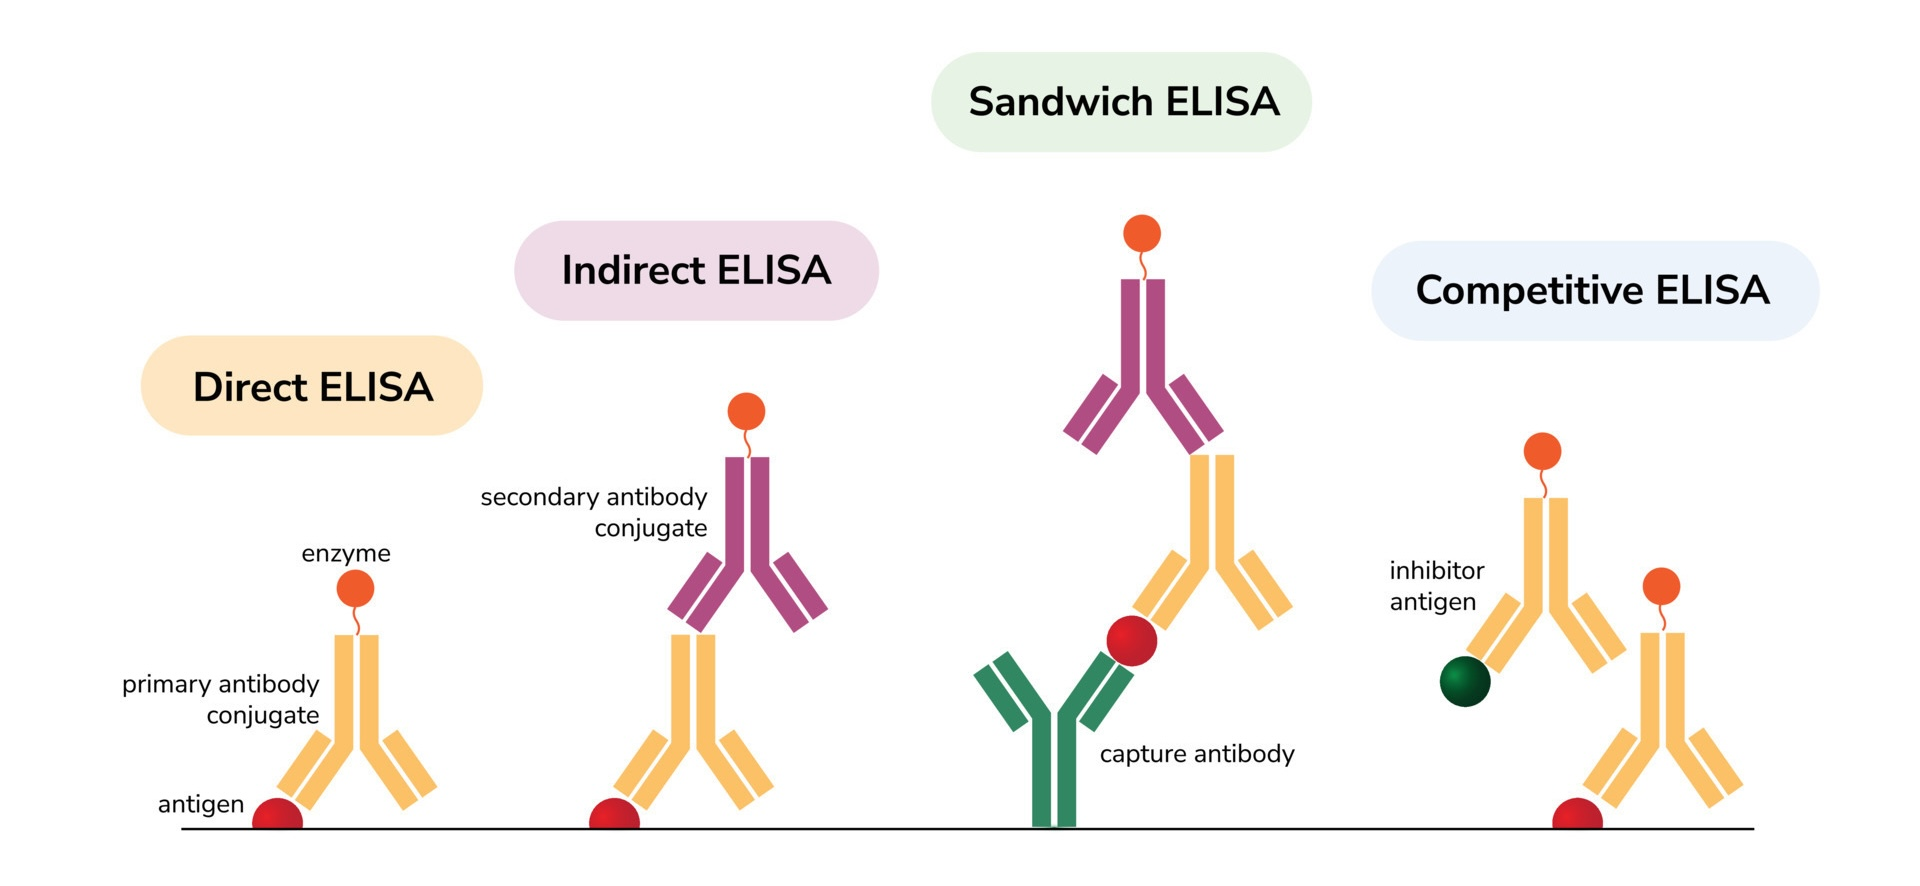
\includegraphics[width=0.95\textwidth]{figures/methods/elisa_types.jpg}
  \caption{四种ELISA类型示意。直接、间接、夹心和竞争ELISA在抗原固定、抗体识别和酶标读出方式上不同，均把抗原--抗体结合转换为酶促信号。图片来源vecteezy。}
  \label{fig:elisa-types}
\end{figure}

\subsection{HBc直接包被ELISA}

HBc直接包被ELISA用于观察preS能否与固定化HBc结合。实验中先将HBVCp149直接吸附到酶标板，封闭后加入带标签的preS蛋白，再用抗标签抗体和显色体系读取板上preS信号。

先对HBVCp149包被浓度进行滴定，并用Langmuir单点吸附模型拟合总信号和特异信号，据此选择后续实验的工作包被浓度。随后在固定HBVCp149的条件下滴定preS，同时设置无HBc包被对照，用来区分HBc依赖性信号和preS或抗体带来的非特异吸附背景。

\subsection{StrepXT捕获preS ELISA}

StrepXT捕获preS ELISA用于调整preS在固相表面的取向。实验时先用StrepXT包被酶标板，封闭后加入带Strep标签的preS蛋白，使preS通过标签被定向捕获；随后加入HBVCp149，并利用抗HBc抗体读取与preS结合的核心蛋白信号。

实验流程先优化StrepXT包被和preS捕获条件，再对preS进行浓度滴定，并用Langmuir模型拟合捕获曲线。根据preS捕获饱和趋势确定工作浓度后，继续滴定HBVCp149，比较实验组与无preS对照组的信号差异。为提高核心蛋白检测灵敏度，后续实验以纯化得到的抗HBc IgG D4替代初始检测抗体。

\subsection{抗HBc Fab捕获HBc ELISA}

抗HBc Fab捕获HBc ELISA用于改善HBc固定化方式。实验中先将抗HBc Fab包被于酶标板，再加入HBVCp149，使核心颗粒由抗体捕获；随后加入preS蛋白，并通过抗GST抗体检测preS信号。该构型避免HBc直接吸附到塑料表面，理论上更有利于保留核心颗粒构象。

实验中先滴定HBVCp149以确定Fab捕获效率和合适核心蛋白浓度，再在固定HBc条件下滴定preS，并设置无HBc和仅HRP对照等对照以评估背景来源。

\begin{figure}[htbp]
  \centering
  \begin{minipage}{0.42\textwidth}
    \centering
    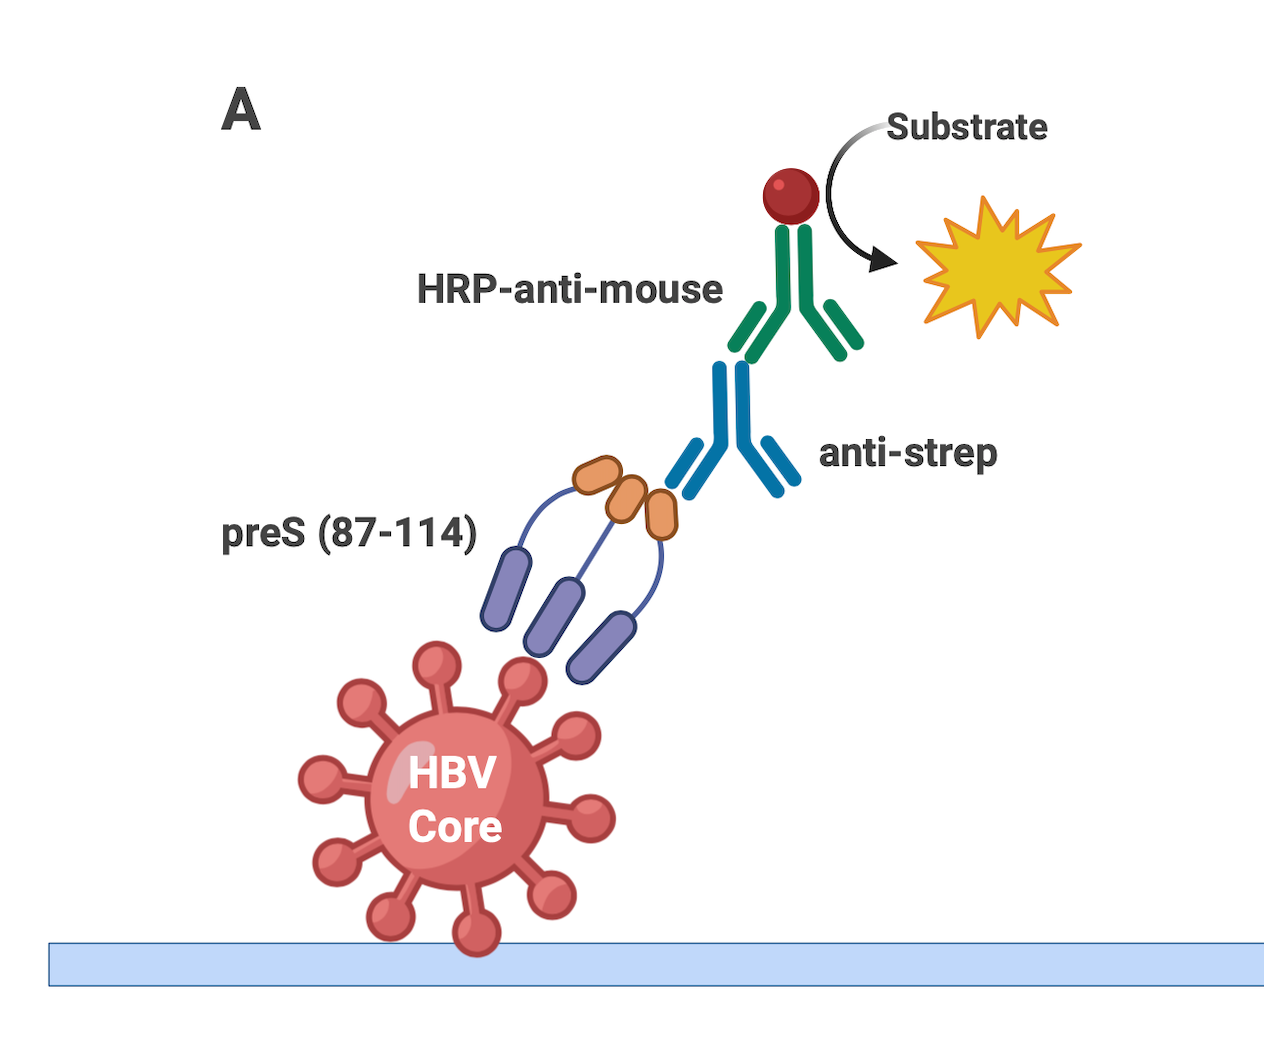
\includegraphics[width=\textwidth]{figures/methods/elisa_a.png}
  \end{minipage}
  \hspace{0.07\textwidth}
  \begin{minipage}{0.42\textwidth}
    \centering
    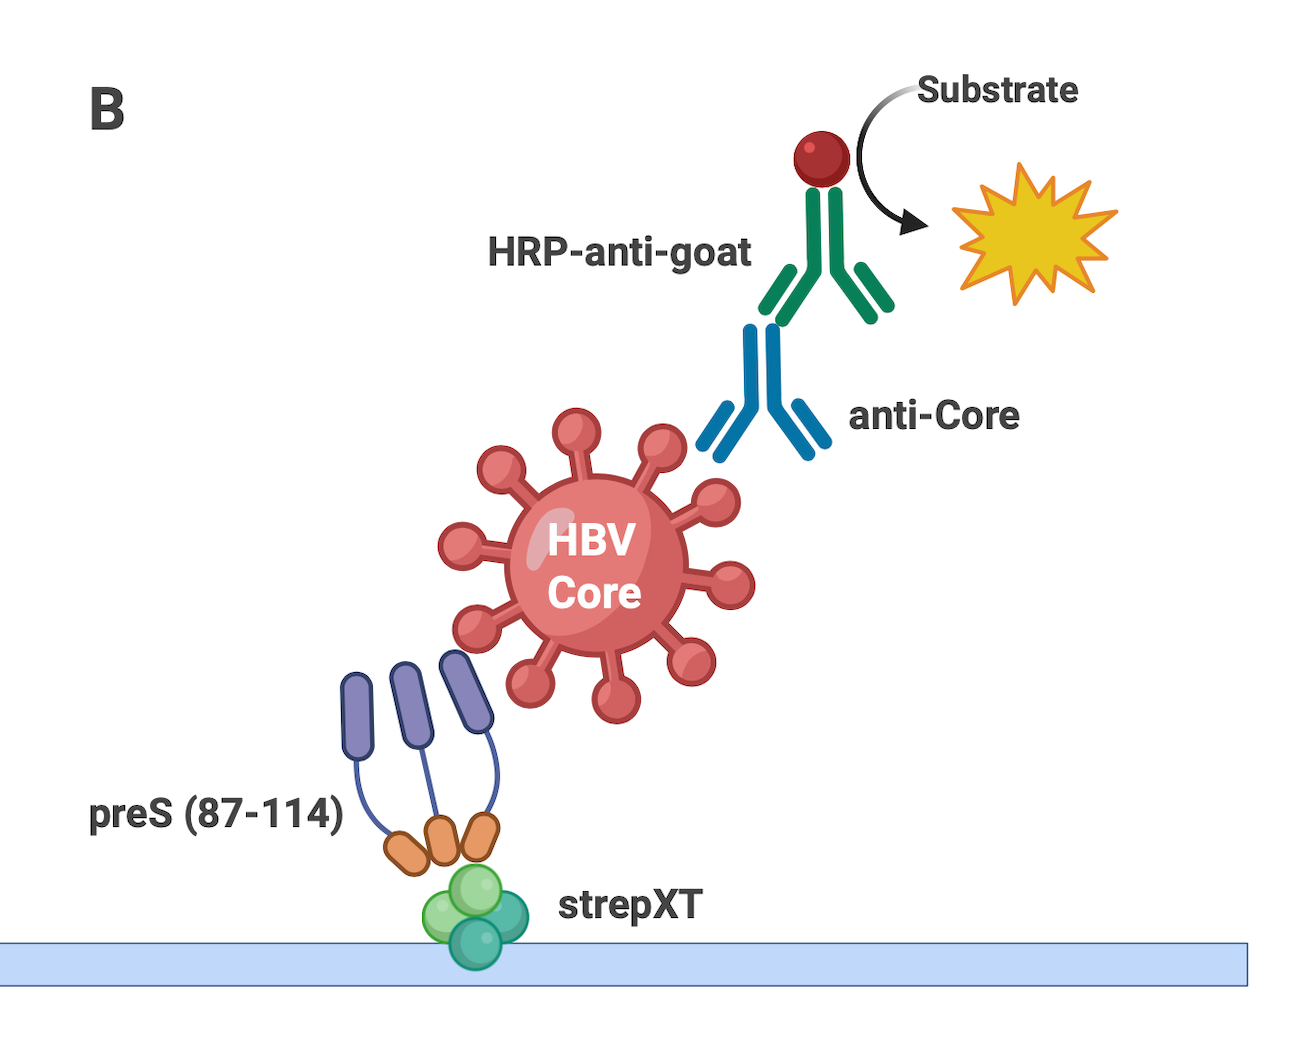
\includegraphics[width=\textwidth]{figures/methods/elisa_b.png}
  \end{minipage}
  \par\medskip
  \begin{minipage}{0.46\textwidth}
    \centering
    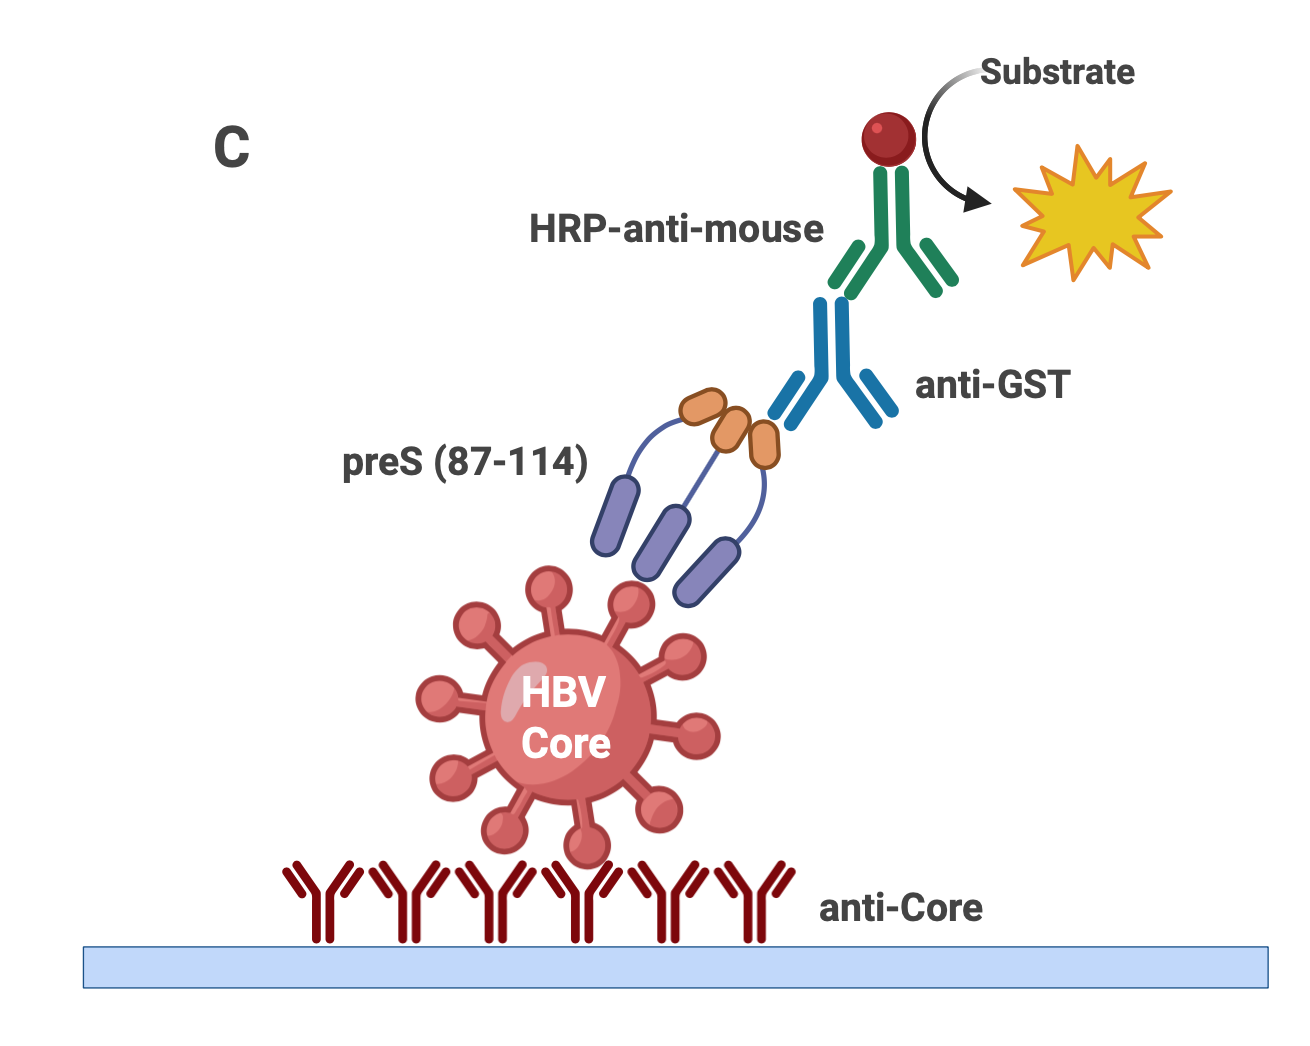
\includegraphics[width=\textwidth]{figures/methods/elisa_c.png}
  \end{minipage}
  \hspace{0.04\textwidth}
  \begin{minipage}{0.42\textwidth}
    \centering
    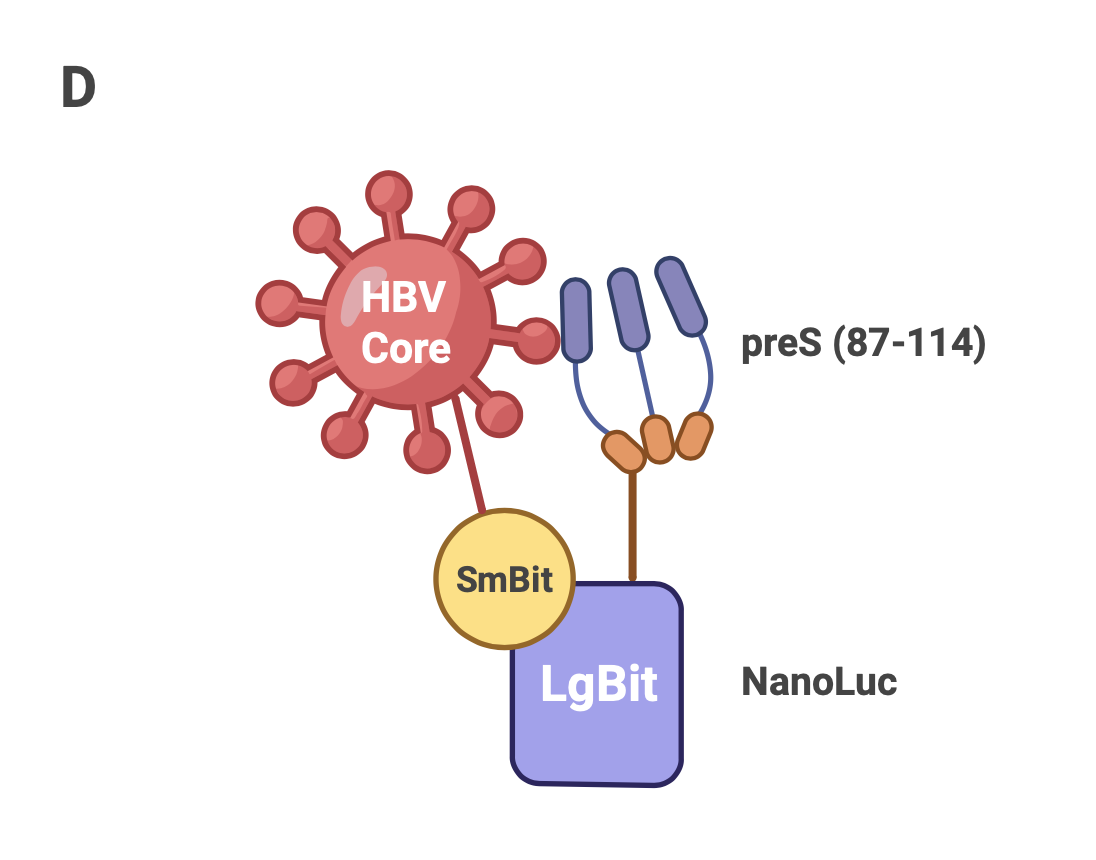
\includegraphics[width=\textwidth]{figures/methods/nanobit.png}
  \end{minipage}
  \caption{HBc--preS相互作用检测模式。A，HBc直接包被ELISA：HBVCp149固定于酶标板，再加入preS 87--114融合蛋白，并通过抗标签抗体及HRP显色体系检测preS信号。B，StrepXT捕获preS ELISA：StrepXT固定在板面后捕获带Strep标签的preS 87--114融合蛋白，再加入HBVCp149，并通过抗HBc抗体及HRP显色体系检测核心蛋白信号。C，抗HBc Fab捕获HBc ELISA：抗HBc Fab固定于酶标板并捕获HBVCp149，再加入preS 87--114融合蛋白，并通过抗GST抗体及HRP显色体系检测preS信号。D，NanoBiT发光互补检测：SmBiT位于HBVCp182侧，LgBiT位于preS 87--114侧；二者接近时恢复NanoLuc活性，加入底物后产生发光信号。}
  \label{fig:method-assay-formats}
\end{figure}

\section{NanoBiT发光互补检测}

\subsection{NanoBiT技术原理}

NanoBiT是一种基于NanoLuc荧光素酶拆分互补的蛋白相互作用检测技术。NanoLuc是一种小分子、单体化且发光强度较高的工程化荧光素酶，可催化furimazine氧化生成furimamide、二氧化碳和光信号。Dixon等利用NanoLuc体积小和发光强的特点，将其工程化拆分为两个互补片段：较大的LgBiT片段约18 kDa，较小的SmBiT片段为11个氨基酸、约1.3 kDa\cite{dixon2016nanoluc}。LgBiT与SmBiT单独存在时自发亲和力较弱；当二者分别融合到两个待测蛋白上，并因目标蛋白相互作用而靠近时，LgBiT和SmBiT可发生结构互补，重新形成具有催化活性的NanoLuc复合物，加入底物后产生发光信号。

\begin{figure}[htbp]
  \centering
  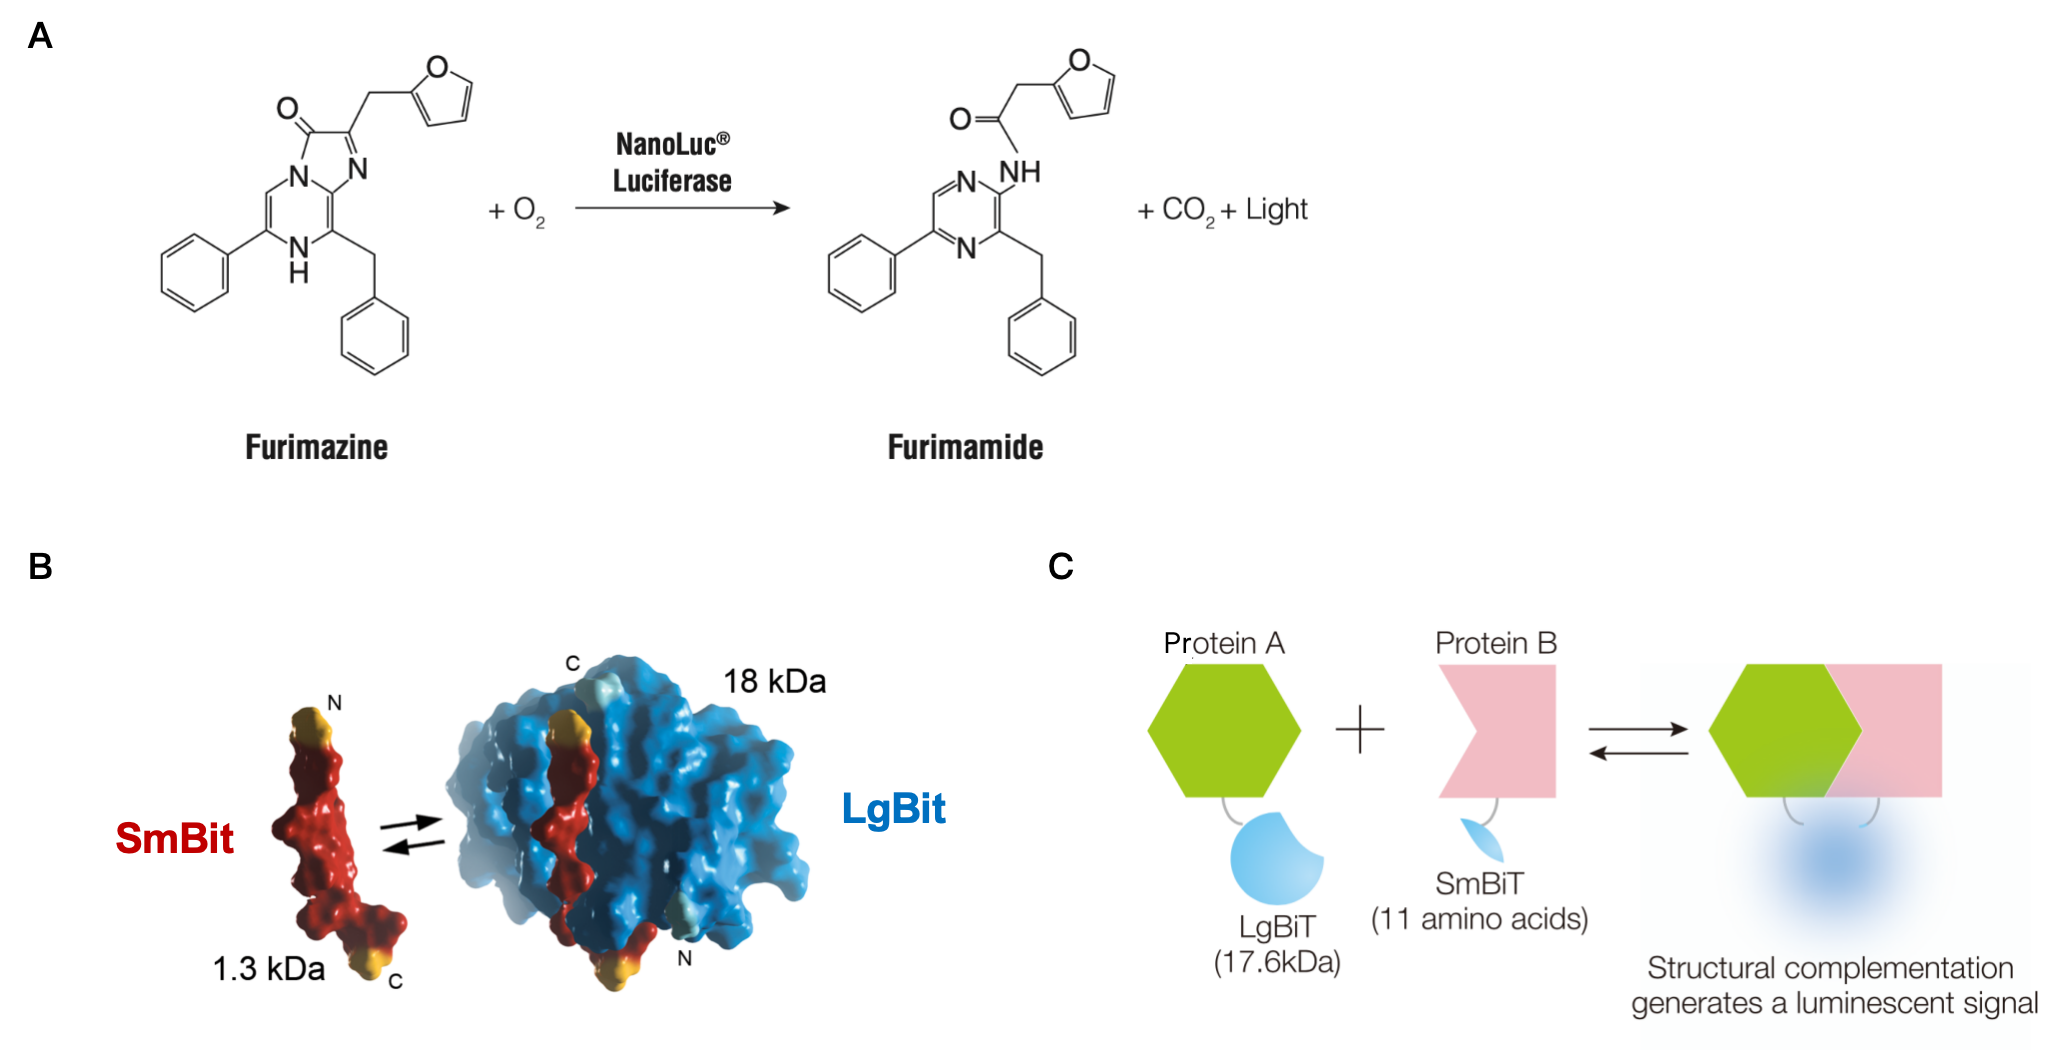
\includegraphics[width=0.75\textwidth]{figures/introduction/nanobit_principle.png}
  \caption{NanoLuc与NanoBiT蛋白互补技术原理。A，NanoLuc催化furimazine氧化并产生发光信号。B，NanoBiT由SmBiT和LgBiT组成，二者互补后恢复NanoLuc活性。C，SmBiT和LgBiT分别融合到两个待测蛋白上时，目标蛋白靠近可带来发光信号。\cite{dixon2016nanoluc}。}
  \label{fig:nanobit-principle}
\end{figure}

与传统亲和沉淀、免疫共沉淀或ELISA相比，NanoBiT读数来自两个融合蛋白在溶液或细胞环境中的空间接近，不必把相互作用完全限制在固相表面。检测过程中也不需要多轮洗涤，因此更接近溶液状态，适合观察HBc--preS这类较弱、可逆且可能受固定化影响的相互作用。Dixon等测得NanoBiT片段自身的本征亲和力约为190 \textmu M，互补过程具有可逆性；这一设计可降低报告片段自身结合对待测蛋白相互作用的驱动作用\cite{dixon2016nanoluc}。NanoLuc体系发光强、背景低、线性范围宽，便于在多孔板中做定量检测和候选调节因子筛选。

\subsection{NanoBiT构建体设计}

构建体设计时，较大的LgBiT不放在HBc侧，以免干扰HBc组装。本研究把较小的SmBiT融合至HBVCp182，把LgBiT接到preS 87--114片段一侧。实验组为HBVCp182-SmBiT与LgBiT-preS 87--114组合；阴性对照为HBVCp182-SmBiT与不含preS的LgBiT融合蛋白组合；阳性对照利用GST标签二聚化特性，将GST-SmBiT与GST-LgBiT相关蛋白组合，用来确认NanoBiT报告系统的检测上限。需要说明的是，NanoBiT信号本质上反映融合蛋白之间的近距离互补，因此仍需结合阴性对照、标签方向、蛋白质量控制以及小分子对发光体系本身影响的排查，再谨慎解释HBc--preS相互作用或其抑制效应。

\subsection{NanoBiT发光检测流程}

NanoBiT检测在白色384孔板中进行。实验前将LgBiT融合蛋白和SmBiT融合蛋白分别用TBS稀释为合适浓度。常规反应中，将10 \textmu L LgBiT融合蛋白与10 \textmu L SmBiT融合蛋白混合，使总体积为20 \textmu L。混合后短暂离心，并在室温孵育约10 min。随后加入20 \textmu L新鲜配制的Nano-Glo底物工作液，底物与缓冲液按1:50配制。加样后振荡约10 s，在室温孵育3--5 min，并使用酶标仪读取发光信号，积分时间设为1000 ms。

初始NanoBiT实验中，LgBiT与SmBiT蛋白按1:1浓度比例混合，以判断实验组、阴性对照和阳性对照之间是否存在可分辨信号。优化实验中固定HBVCp182-SmBiT的终浓度，并滴定LgBiT-preS或LgBiT阴性对照蛋白。

\section{小分子抑制、突变体比较与数据分析}

\subsection{小分子抑制实验}

小分子抑制实验用于评估候选分子是否改变HBc--preS相关NanoBiT信号。本文检测Triton X-100（TX100）、NP-40和香叶醇。在含foldon三聚化结构域的体系中，根据NanoBiT滴定结果选择40 nM GST-LgBiT-preS 87--114-foldon-strep-His作为初筛工作浓度，并使用相同浓度的GST-LgBiT-foldon-strep-His作为阴性对照。初筛时，将小分子按浓度梯度加入NanoBiT反应体系后读取发光信号。由于直接加药条件下抑制趋势不够稳定，后续改为先将小分子与HBVCp182-SmBiT预孵育约2 h，再加入LgBiT-preS或LgBiT阴性对照检测，并适当提高小分子浓度范围。分析这些结果时，同时考虑溶剂背景、高浓度去垢剂对蛋白稳定性、NanoBiT片段互补、底物发光反应和体系浊度的影响。

为降低foldon三聚化结构域带来的多价效应，后续构建并制备不含该结构域的GST-LgBiT-preS 87--114-His和GST-LgBiT-His。该体系主要用于观察去除foldon三聚化结构域后NanoBiT信号窗口如何变化，并作为preS突变体比较的基础；本文的小分子表观抑制结果仍主要基于含foldon三聚化结构域的构建体解释。实验中同步检测实验组和阴性对照组，分析时扣除或比较阴性对照背景，以判断小分子对HBc--preS相关信号的影响。

\subsection{preS突变体结合能力比较}

为检验结构模型中关键残基对HBc结合的贡献，本研究比较野生型（wild-type）preS 87--114及R102A、H105A和W111A突变体的NanoBiT信号。由于foldon三聚化结构域和GST标签可能带来多价结合或非目标性二聚化，突变体比较优先使用去除foldon三聚化结构域后的LgBiT-preS蛋白。实验中固定HBVCp182-SmBiT，滴定不同LgBiT-preS突变体蛋白，并设置LgBiT阴性对照。通过比较同一浓度范围内的发光信号强度和相对趋势，评估各残基对HBc--preS相互作用的影响。

\subsection{数据处理与评价指标}

ELISA和NanoBiT实验均设置实验组、阴性对照和必要的背景对照。对于浓度滴定实验，首先计算各条件下重复孔的平均值和标准差；除特别说明外，图中误差线表示同一实验内重复孔的标准差。随后根据实验设计扣除无核心蛋白、无preS或不含preS的LgBiT阴性对照背景，得到特异性信号。对呈饱和趋势的结合曲线，可采用Langmuir单点结合模型进行拟合，以描述信号随蛋白浓度增加逐渐接近平台的趋势。由于NanoBiT读数同时受到融合蛋白空间接近、片段互补效率和标签多聚化状态影响，拟合参数仅作为当前检测构型下的表观参数，不直接等同于热力学解离常数。

检测体系的统计学窗口使用Z-factor评价。Z-factor同时考虑实验组与阴性对照之间的均值差异和组内波动，可反映检测体系是否具备稳定筛选能力，其计算公式如下\cite{zhang1999simple}：
\begin{equation}
  Z = 1 - \frac{3\left(\sigma_{\mathrm{exp}}+\sigma_{\mathrm{neg}}\right)}
  {\left|\mu_{\mathrm{exp}}-\mu_{\mathrm{neg}}\right|}.
  \label{eq:z-factor}
\end{equation}
其中，$\mu_{\mathrm{exp}}$和$\sigma_{\mathrm{exp}}$分别表示实验组信号的平均值和标准差，$\mu_{\mathrm{neg}}$和$\sigma_{\mathrm{neg}}$分别表示阴性对照信号的平均值和标准差。通常Z-factor大于0.5说明检测窗口较好，可用于较稳健的定量比较；0--0.5提示体系处于边界状态；小于0则说明实验组和对照组分离不足或波动过大。Z-factor反映筛选窗口质量，不能单独证明分子机制。小分子抑制实验中，若高浓度小分子同时改变阴性对照信号、阳性互补信号或底物背景，则不直接计算IC$_{50}$，仅进行趋势性分析，并把背景变化列为后续优化内容。
